\chapter{The Standard Model and Beyond}
\label{chap:SM&beyond}

\section{The Standard Model}
\label{sec:SM}

% SM as best theory framework
% Composition of SM
The Standard Model (SM) of particle physics is our current best framework describing the fundamental constituents of the universe, as well as three out of the four known fundamental forces of nature, namely the weak, strong, and electromagnetic forces. In this framework, seventeen particles are described through quantum field theory. The particles that make up the SM are listed in Figure \ref{fig:sm-table}.

\begin{figure}
    \centering
    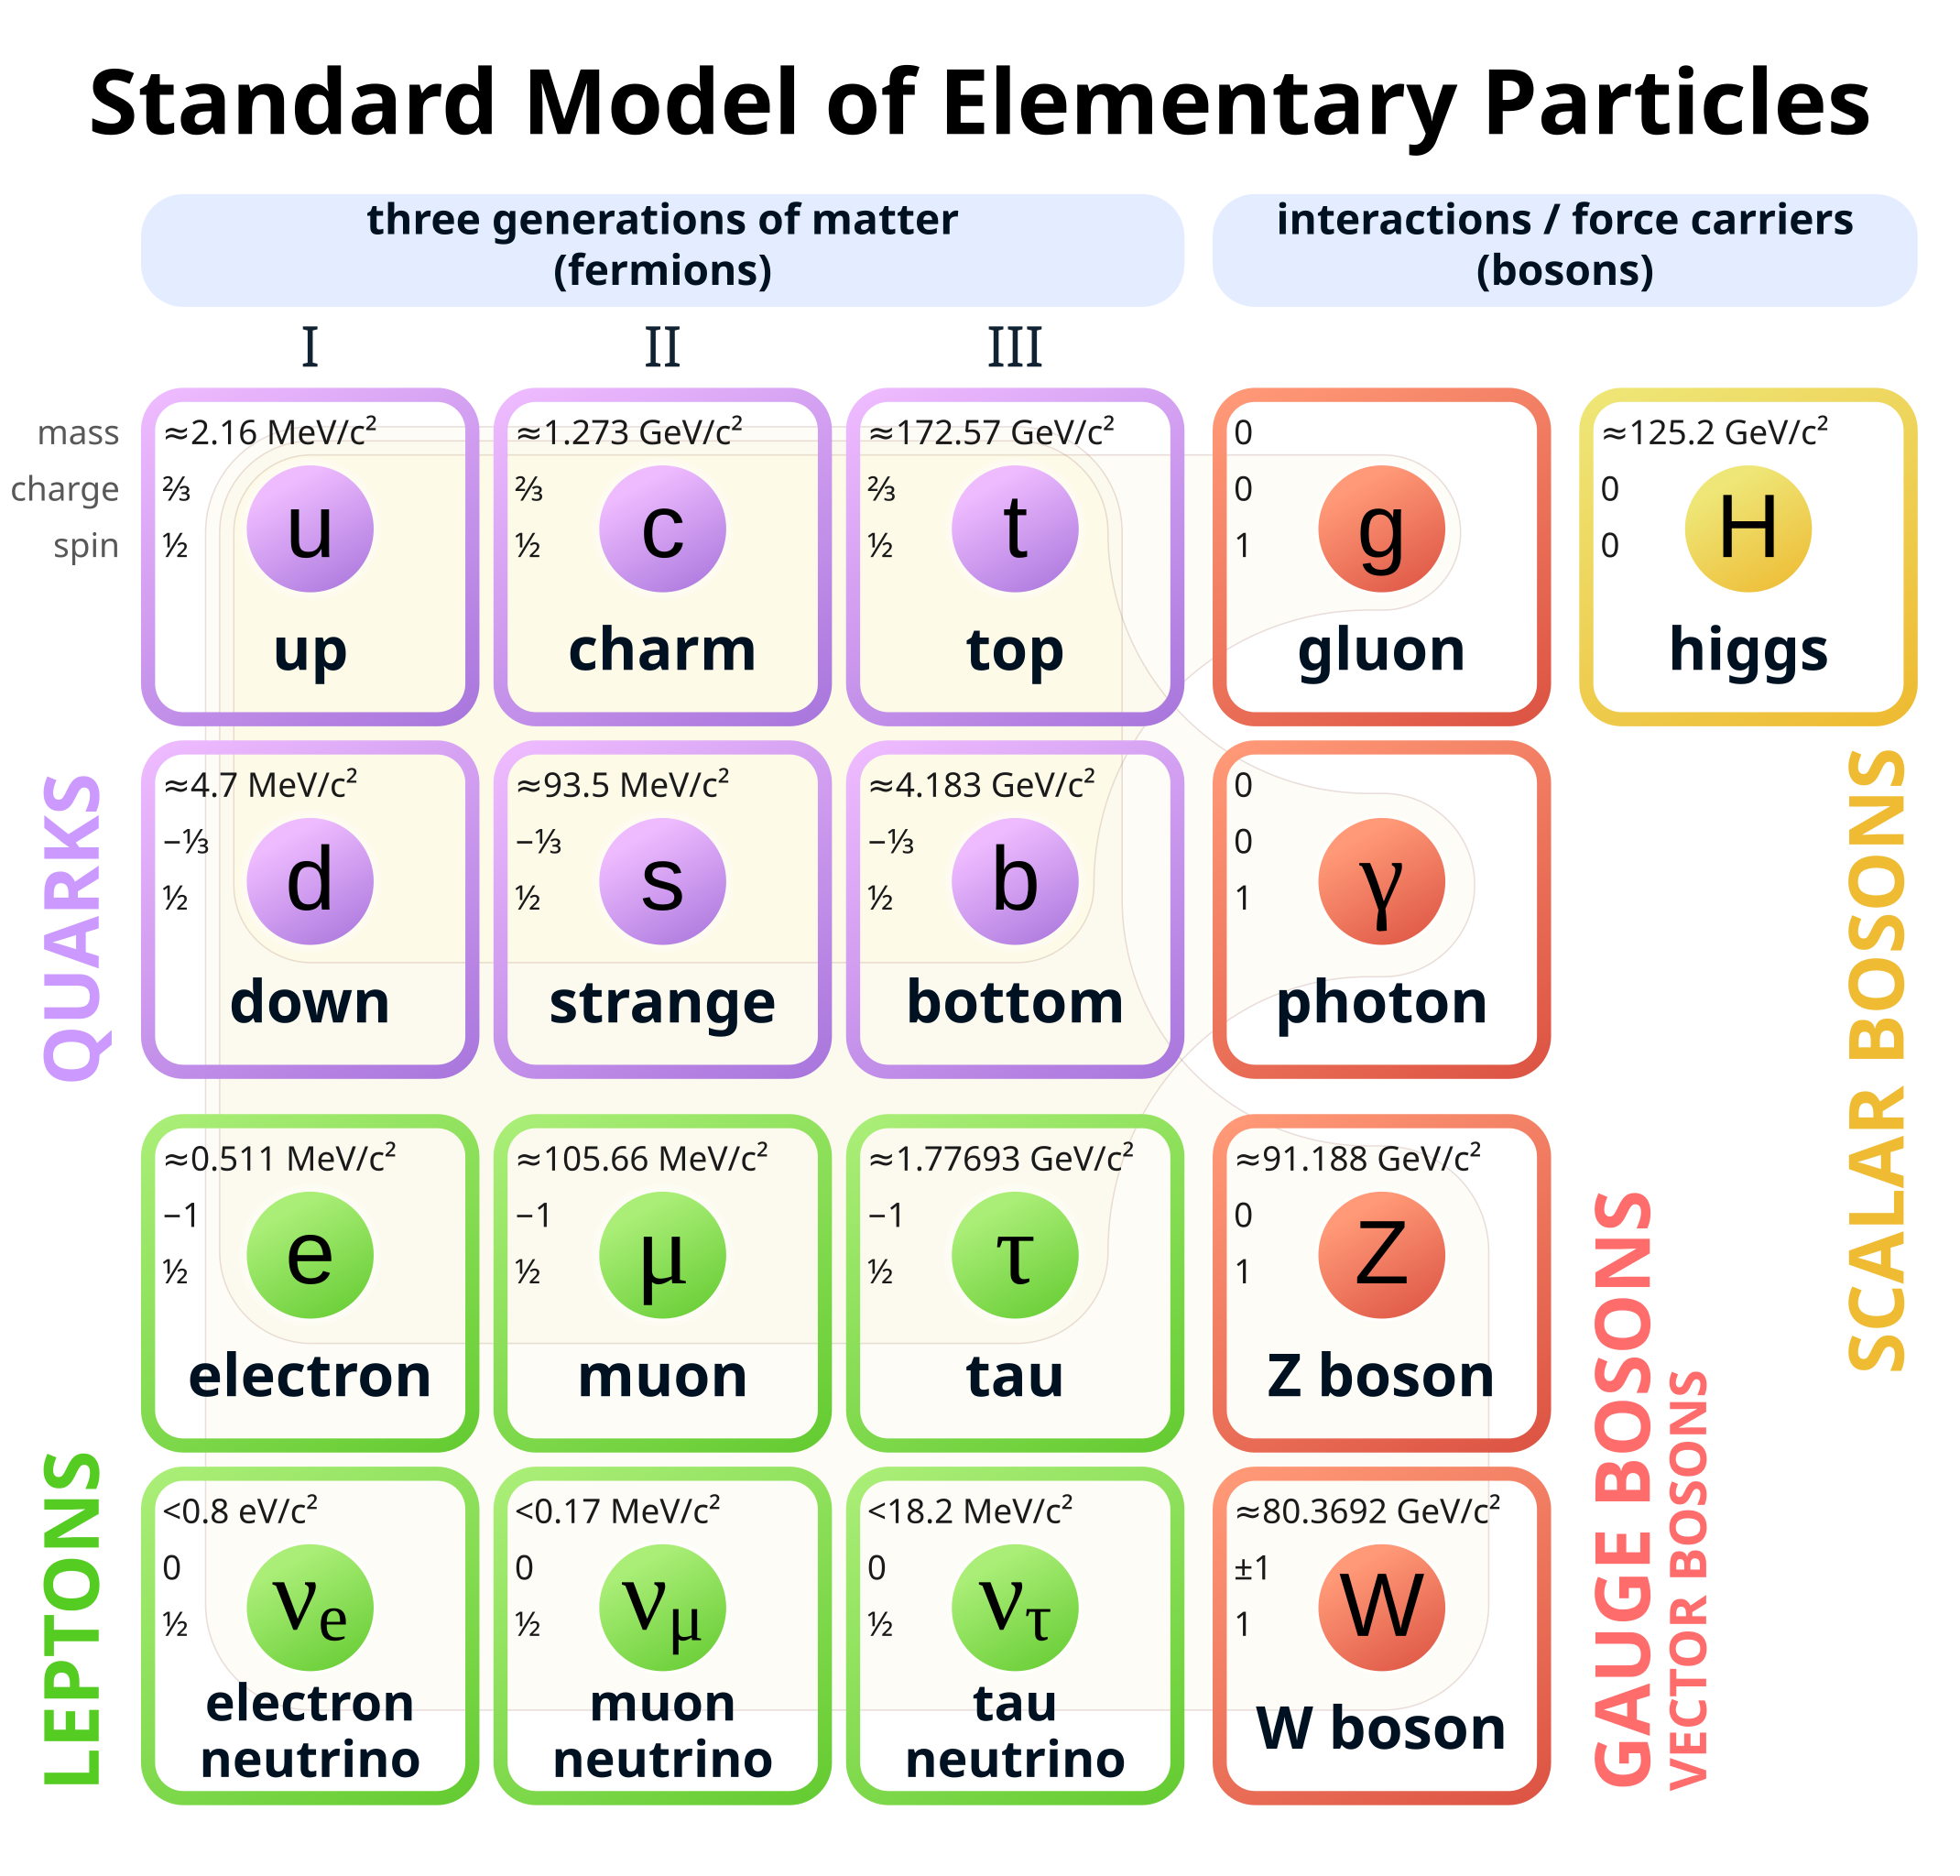
\includegraphics[width=0.5\linewidth]{images/sm.png}
    \caption{Particles that make up the Standard Model as well as their charge, spin and mass \cite{smwiki}}
    \label{fig:sm-table}
\end{figure}

In the SM, there are twelve fermions with spin-$\frac12$. Of these twelve, six are the quarks. These particles interact through strong force as well as through electromagnetic force, given that they carry an electric and a color charge. In addition, there are six leptons, but only the electron, muon and tau carry electric charge. However, the corresponding neutrinos have very low mass and are electrically neutral. 

In addition to the fermions, there are five bosons in the SM, four of which, the vector bosons, are responsible for three of the four known fundamental forces. The gluon, which carries color charge but is electrically neutral and is responsible for the strong force. The photon is massless and carries no charge, and is responsible for the electromagnetic force. Finally, the $Z$ and $W$ bosons are responsible for the weak force. In addition to these forces, carriers, there is a singular spin-0 boson, the Higgs boson. Through interactions with this particle, all massive particles in the Standard Model acquire their mass.

Each of these particles is associated with quantum field theory. The spin-1 gauge bosons are described by fields that transform as Lorentz 4-vectors. For the strong force, the quantum field theory is quantum chromodynamics (QCD). This theory, which is an $\text{SU}(3)$ Yang-Mills theory, describes the interactions between quarks and gluons, as well as the self-interactions of gluons. The Lagrangian that describes these interactions is

\begin{align}
    \mathcal L\subset \sum_q \bar{\psi}_{q,a}\left(i\gamma^\mu \partial_\mu \delta_{ab} - g_s\gamma^\mu t_{ab}^C \mathcal A_\mu^C\right)\psi_{q,b} - \frac14 F^{A}_{\mu\nu}F^{A\mu\nu}
\end{align}

where $\psi_{q,a}$ is the quark field for flavor $q$ and color index $a$, $g_s$ is the strong coupling constant, $t_{ab}^C$ is the generator $\text{SU}(3)$ in fundamental representation, $A_\mu^C$ is the gluon field with color index $C$ and $F_{\mu\nu}^A$ is the gluon field strength tensor. For its part, the aforementioned term is written as:

\begin{align}
    F^A_{\mu\nu} = \partial_\mu \mathcal A_\nu^A - \partial_\nu\mathcal A_\mu^A - g_s f_{ABC}\mathcal A_\mu^B\mathcal A_\nu^C.
    \label{eq:qcd-tensor}
\end{align}

where $f^{ABC}$ are the structure constants of the $\text{SU}(3)$ group that determine how the gluons interact with each other. It is precisely the latter term in \ref{eq:qcd-tensor} that is responsible for gluon self-interaction, and it leads to three and four-gluon vertices. This peculiarity, which is a product of the non-Abelian nature of the QCD gauge group, leads to an energy potential which rises with distance, unlike the electromagnetic force which has a falling energy potential. As a result, at larger distances, the production of quark-antiquark becomes favorable, leading to color-neutral final states, i.e. confinement.

In high-energy particle collisions, such as those occurring in the Large Hadron Collider between protons, high momentum transfer results in the separation of quarks and gluons. Due to color confinement and the increasing nature of the strong force energy potential with distance, this results in spontaneous quark-antiquark pair generation. The high energy of the initial collision is imparted on the newly created particles, which may also lead to further pair production of quarks, until the resulting final state is color neutral. This chain process of hadronization until all quarks are confined in color-neutral bound states leads to collimated showers of particles called jets. 

% In high-energy particle physics, 'jets' refer to collimated sprays of particles that result from the hadronization of quarks and gluons. These jets are produced in particle collisions, especially in processes involving quantum chromodynamics (QCD), such as those taking place in particle accelerators.

% - **Color Confinement**: Color confinement is a phenomenon where quarks and gluons are never found in isolation (free state). Instead, they exist only within hadrons due to the nature of the strong force, governed by QCD. When high-energy collisions occur, quarks and gluons are knocked out of protons or neutrons and try to move apart. However, as they separate, the strong force between them does not diminish, leading to the creation of new quark-antiquark pairs. This process results in jets, as chain reactions continue until all quarks are confined in hadrons.

% - **Coupling Constant of the Strong Force**: The strength of the strong force is described by the coupling constant, which 'runs' or varies with the energy scale due to asymptotic freedom. At high energies, this coupling constant decreases, making quarks and gluons behave almost freely (perturbative regime). As the energy scale lowers, the coupling increases, illustrating confinement and requiring non-perturbative methods for analysis.

% - **Perturbation vs Non-Perturbation in QCD**: In QCD, perturbative calculations are applicable when the running coupling constant is small (at short distances/high energies), enabling the use of standard perturbation theory. Non-perturbative methods become necessary at lower energies/large distances, where the coupling constant grows, and confinement dominates, necessitating techniques like lattice QCD to study phenomena like jet formation.

\section{Dark Matter}
\label{sec:DM}

% Since the time of Oort and Rubin's evidence has been mounting in favor of the existence of this illusory type of matter. Alongside this evidence, there have been a multitude of proposed models\footnote{Description of this evidence, as well as some of the proposed models, can be found in Section \ref{sec:DM}.}. In this work, we consider a class of DM models that propose that it is composed of stable dark baryons in a confining Hidden Valley sector that interacts with the SM only through a mediator. If we assume the cogeneration of dark matter and baryonic matter in the early universe through the same mechanism, then we could simultaneously explain the matter-antimatter asymmetry, the dark matter abundance, and the coincidence of mass and number density of DM and baryonic matter\cite{schwallerEmergingJets2015}. Moreover, this class of models would be consistent with astronomical observations indicating that dark matter is cold and has large self-interactions.

Although the predictive power of the SM has been shown repeatedly, there have been many signs of its incompleteness. One particularly compelling case is that of DM. Evidence of its existence dates back to the 1940's with J.H. Oort's observations that the velocity distribution of stars in the Milky Way would lead to stars moving fast enough to escape \cite{oortProblemsConcerningStructure1940}, as well as in the 1980s with V. Rubin's studies on the rotation curves of 60 galaxies which showed that the mass distrubution of galaxies extends beyond what can be accounted for through visible matter only \cite{rubinDarkMatterSpiral1983}.

The evidence for dark matter is not limited to the rotation curves of galaxies. The relatively small scale of the anisotropies observed in the Cosmic Microwave Background (CMB) by COBE (COsmic Background Explorer) are too small to have been the seeds of the formation of large-scale structures in the universe. There must have been charge-neutral matter that was able to start the structural formation before recombination occurred in the early universe. Additionally, precision studies of the CMB fluctuations carried out using WMAP (Wilkinson Microwave Anisotropy Probe) have indicated that the total matter density of the universe is $\Omega_{m}h^2 = 0.1334$, and that only a small fraction of this, $\Omega_{b}h^2 = 0.02260$, is attributable to baryonic matter. The rest, $\Omega_{dm}h^2 = 0.1123$ or about $83\%$ of the total mass density, comes from elusive dark matter. Thus, a substantial amount of the universe's content is nonbaryonic and not described by the SM.

Numerous models have been proposed to extend the SM to accommodate DM. Among them are supersymmetry and WIMPs, but no signs of these have been observed. Another class of models of particular interest in this work are those that propose that dark matter is composed of stable dark baryons in a confining Hidden Valley sector that interacts with the SM only through a mediator. If we assume the cogeneration of dark matter and baryonic matter in the early universe through the same mechanism, then we could simultaneously explain the matter-antimatter asymmetry, the dark matter abundance, and the coincidence of mass and number density of DM and baryonic matter. Moreover, this class of models would be consistent with astronomical observations indicating that dark matter is cold and has large self-interactions.


\section{Emerging Jets}
\label{sec:EMJs}

Experimental searches have excluded many DM models with weakly interacting massive particles. As a result, alternate models have emerged with a hidden guage sector with strong self-interactions in this hidden dark sector. In this work, we consider a class of models first proposed in \cite{schwallerEmergingJets2015}, which extends the Standard Model by including a confining, QCD-like dark sector of particles which are charged under a new gauge group with a non-abelian gauge symmetry, extending the SM to:

\begin{equation}
	\begin{aligned}
		G_{\text{SM}} \times \text{SU}(N_d).
	\end{aligned}
\end{equation}

This dark sector is composed of $n_f$ dark quarks, $Q_d$, which are Dirac fermions, and are singlets under the SM gauge group, but charged under the new $SU(N_d)$ gauge group with $N_d \geq 2$ dark colors. Given that this new sector is confined with a confinement scale $\Lambda_d$, the dark quarks would hadronize into dark mesons and baryons, which are bound states of the dark quarks. The dark baryons would carry a conserved charge, namely the dark baryons number, which means that the lightest dark baryons, the equivalent of the dark proton, would be stable and thus serve as the dark matter candidate put forward by this model. Dark mesons, on the other hand, would not carry such a charge, and would be unstable, capable of decaying back into SM particles.

We consider two possible scenarios for the mediator between the dark sector and the SM. Firstly, we consider a bifundamental scalar mediator $X_{\text{dark}}$, charged under $SU(N_d)$ and QCD. The decay of such a mediator would produce a quark, dark quark pair. The SM quarks would hadronize and produce a jet in the SM, and the dark quark would produce a dark jet. The dark jet would be composed of dark baryons, the lightest of which, the dark sector equivalent of the proton, would be stable and thus serve as the dark matter candidate put forward by this model, and dark mesons. The dark mesons, on the other hand, if kinematically allowed, would decay to the model's lightest composite state, i.e. the dark pion. This meson would itself be unstable and, assuming a large energy hierarchy between the mediator mass and the confinement scale of the dark sector, that is, $m_{\pi_{\text{DK}}} \gg \Lambda_d$, could potentially travel macroscopic distances before decaying back into SM particles. Because the decay of these unstable dark mesons is a stochastic process, they would happen at different positions in the detector, and thus the energy of the dark jet would emerge into the detector. This would then be seen in the detector as a wide jet with displaced vertices. We call these types of objects emerging jets (EMJs). In this work, we focus on the pair production of this bifundamental mediator through gluon-gluon fusion or quark-antiquark annihilation. The Feynman diagrams for these processes can be seen in Figure \ref{fig:t-chan}.
\vspace{0.2in}

\begin{figure}[h] % TODO
	\centering
	\begin{subfigure}{0.45\textwidth}
		\begin{fmffile}{feyn_t_channel1}
            \begin{fmfgraph*}(200,100)
                \fmfleft{i1,i2}
                \fmfright{o1,o2,o3,o4}

                \fmf{gluon}{i1,v1}
                \fmf{gluon}{i2,v1}
                \fmf{gluon, label=$g$, label.side=right, label.dist=50}{v1,v2}

                \fmflabel{$g$}{i1}
                \fmflabel{$g$}{i2}

                \fmf{dbl_dashes, label=$\text{X}_{\text{dark}}$, l.s=right, tension=1.2}{v2,v3}
                \fmf{dbl_dashes, label=$\text{X}_{\text{dark}}^\dagger$}{v2,v4}

                \fmf{fermion}{o1,v3}
                \fmf{fermion}{v3,o2}

                \fmf{fermion}{o3,v4}
                \fmf{fermion}{v4,o4}

                \fmflabel{$Q$}{o1}
                \fmflabel{$\bar q$}{o2}
                \fmflabel{$q'$}{o3}
                \fmflabel{$\bar{Q}'$}{o4}
            \end{fmfgraph*}
            \end{fmffile}
	\end{subfigure}
	\hfill
        \centering
	\begin{subfigure}{0.45\textwidth}
		\begin{fmffile}{feyn_t_channel2}
            \begin{fmfgraph*}(200,100)
                \fmfleft{i1,i2}
                \fmfright{o1,o2,o3,o4}

                \fmf{fermion}{i1,v1}
                \fmf{fermion}{v1,i2}
                \fmflabel{$\text{q}$}{i1}
                \fmflabel{$\bar{\text{q}}$}{i2}

                \fmf{gluon, label=g}{v1,v2}

                \fmf{dbl_dashes, label=$\text{X}_{\text{dark}}$, l.s=right, tension=1.2}{v2,v3}
                \fmf{dbl_dashes, label=$\text{X}_{\text{dark}}^\dagger$}{v2,v4}

                \fmf{fermion}{o1,v3}
                \fmf{fermion}{v3,o2}

                \fmf{fermion}{o3,v4}
                \fmf{fermion}{v4,o4}

                \fmflabel{$Q$}{o1}
                \fmflabel{$\bar q$}{o2}
                \fmflabel{$q'$}{o3}
                \fmflabel{$\bar{Q}'$}{o4}
            \end{fmfgraph*}
            \end{fmffile}
	\end{subfigure}
	\caption{Feynman diagrams for pair production of $X_{\text{dark}}$ mediators via gluon-gluon fusion (left) and quark-antiquark annihilation (right), with each mediator decaying to an SM quark and a dark quark.}
	\label{fig:t-chan}
\end{figure}

The other type of model considered in this work is one in which the mediator is a neutral vector boson $Z_{\text{dark}}$. This mediator couples to quarks and dark quarks, enabling the s-channel production of a pair of dark quarks through the annihilation of a pair of quarks, as shown in \ref{fig:s-chan}. This resonant production has a final state with a pair of EMJs produced by the hadronization of the dark quarks.

\begin{figure}[h]
    \centering
    \begin{fmffile}{feyn_s_channel}
    \begin{fmfgraph*}(200,100)
        % Incoming quarks
        \fmfleft{i1,i2}
        \fmfright{o1,o2}
    
        % Internal vertices
        \fmf{fermion}{i1,v1}
        \fmf{fermion}{v1,i2}
    
        \fmf{boson, label=$Z'$}{v1,v2}
    
        % Outgoing dark quarks
        \fmf{fermion}{o1,v2}
        \fmf{fermion}{v2,o2}
    
        % Label the external particles
        \fmflabel{$q$}{i1}
        \fmflabel{$\bar{q}$}{i2}
        \fmflabel{$Q$}{o1}
        \fmflabel{$\bar{Q}$}{o2}
    \end{fmfgraph*}
    \end{fmffile}
    \caption{Feynman diagram for s-channel production of a pair of dark quarks through a $Z'$ mediator}
    \label{fig:s-chan}
\end{figure}

We consider only a version of these models with a simplified flavor-aligned structure of the dark sector quarks, and with only the Yukawa coupling to the $\text{d}$ quark being non-negligible. As discussed in \cite{schwallerEmergingJets2015}, the average decay length of a dark pion in such a model is given by:

\begin{equation}
	\begin{aligned}
		c\tau_{\pi_{\text{dark}}} = 80 \text{ mm} \left(\frac{1}{\kappa^4}\right) \left(\frac{2 \text{ GeV}}{f_{\pi_{\text{dark}}}}\right)^2 \left(\frac{100 \text{ MeV}}{m_d}\right)^2 \left(\frac{2 \text{ GeV}}{m_{\pi_{\text{dark}}}}\right)  \left(\frac{m_{X_{\text{dark}}}}{1 \text{ TeV}}\right)^2
	\end{aligned}
\end{equation}

\noindent where $\kappa$ is the Yukawa coupling between the dark quarks and the mediator, $f_{\pi_{\text{dark}}}$ is the dark pion decay constant, $m_d$ is the down quark mass, $m_{\pi_{\text{dark}}}$ is the dark pion mass, and $m_{X_{\text{dark}}}$ is the mediator mass. 


% \begin{equation}
% 	\begin{aligned}
% 		c\tau_{\pi_{\text{dark}}}^{\alpha\beta} = \frac{
% 		8\pi m_{X_{\text{dark}}}^4
% 		}{
% 		N_c m_{\pi_{\text{dark}}}f^2_{\pi_{\text{dark}}} \sum_{ij}|\kappa_{\alpha i}\kappa_{\beta j}^{*}|^2 (m_i^2 + m_j^2) \sqrt{\left(1 - \frac{(m_i + m_j)^2}{m_{\pi_{\text{dark}}}^2}\right)\left(1-\frac{(m_i - m_j)^2}{m_{\pi_{\text{dark}}}^2}\right)}
% 		}
% 	\end{aligned}
% \end{equation}
